\chapter{Künstliche Neuronale Netze} \label{ANN}

Künstliche Neuronale Netze (engl. artificial neural networks) sind Systeme, die auf dem Gehirn von Tieren und Menschen basieren und besteht aus endlich viele Einheiten, Neuronen. Der Datenaustausch geschieht über gerichtete Verbindungen zwischen den Neuronen. Forscher beschäftigen sich mit Neuronalen Netzen aus unterschiedlichen Gründen. In der Biologie simulieren Forscher diese, um sich den Prozess des Lernens und weitere Mechaniscmen zu untersuchen. In der Informatik wird aber versucht, die Lernfähigkeit des Gehirns nachzubilden und auszunutzen.

In den folgenden Kapiteln wird zuerst auf den Neuronen sowohl in der Biologie als auch in der Künstliche Intelligen eingegangen. Weiterhin werden die Eigenschaften von Neuronalen Netzen erklärt. Zum Schluss stelle ich den Gradientenvarfahren vor, anhand dessen diese Netze lernen.

\section{Biologische Grundlagen}

Das tierische Gehirn leitet jede einzelne Aktivität in dem Körper eines Tieres, inklusive die Verarbeitung von Daten. Laut \cite{GEHIRN:12} besteht das Gehirn aus 86 Milliarden Neuronen, die in Cliquen verbunden sind. Neuronen in einer Clique komunizieren untereinander, indem sie Signale über ihre Axone weiterleiten und Signale über ihren Dendrit empfangen. Eine Verbindung zwischen Neuronen existiert, wenn die Axonterminale eines Neurons den Dendrit eines anderen berührt. Zur Veranschaulichung ist den Aufbau eines Neurons in Abbildung \ref{neuron} gegeben. Jeder Signal wird in dem Soma verarbeitet und durch die Axone weitergeschickt.

\begin{figure}[!htbp]
	\centering
	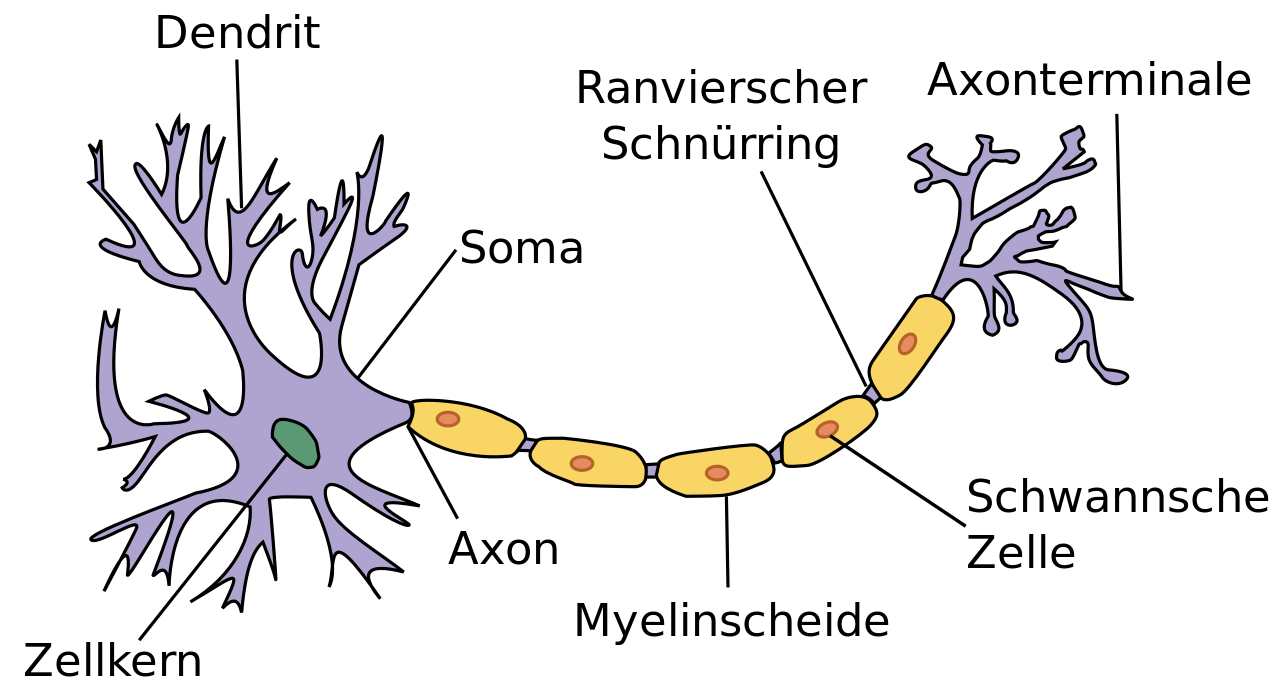
\includegraphics[scale=0.2]{images/Neuron_(deutsch)-1.png}
	\caption{Neuron \cite{NWIKI:19}}\label{neuron}
\end{figure}

Auf dem selben Prinzip funktionieren auch Neuronen in Künstlichen Neuronalen Netzen (KNN). Im folgenden Kapitel wird mehr darauf eingegangen. \cite{NWIKI:19} \cite{GEHIRN:12}

\section{Neuron in Künstlichen Neuronalen Netzen}

Neuronale Netze sind streng genommen gerichtete Graphen, wo jeder Knoten ein Neuron ist und jede Kante eine Verbindung zwischen Neuronen beschreibt. Die Neuronen können in drei Gruppen, oder auch als Schichten (\textit{engl.} Layers) bekannt, unterteilt werden - Eingabe-, Ausgabe- und versteckte Neuronen. Die Ein- und Ausgabeknoten sind die Einheiten, die mit der Umgebung verbunden sind, dabei ist klar welche Knoten was sind. Die übrigen Elemente werden in dem Netz eingebaut und kommunizieren nur mit anderen Neuronen. Daraus ergibt sich auch ihren Namen ``versteckt''.

Jede Verbindung zwischen Neuronen in KNN erhält ein Wert. Der Verbindungswert wird meistens als Gewicht bekannt. Bei einem Gewicht von 0 existiert keine Verbindung zwischen Neuronen. In einem KNN werden nur die Gewichte gelernt, während die Neuronen nur eine mathematische Funktion beschreiben. Eine übliche Repräsentation der Gewichte ist eine Matrix \ref{knnmat}.

\begin{align}
	\label{knnmat}
	\bordermatrix{ 	
			   & u_1 			& u_2			 & \dots & u_r			    \cr
		u_1    & w_{u_{1}u_{1}} & w_{u_{1}u_{2}} & \dots & w_{u_{1}u_r}		\cr
		u_2	   & w_{u_{2}u_{1}} & w_{u_{2}u_{1}} & 	     & w_{u_{2}u_{1}}	\cr
		\vdots & \vdots	      	& 			     &       & \vdots			\cr
		u_r    & w_{u_{r}u_{1}} & w_{u_{r}u_{2}} & \dots & w_{u_{r}u_r}  	\cr 
	}
\end{align}

Die Beziehungen zwischen Neuronen aus zwei Schichten wird außerdem ganz gut in der Matrix dargestellt. Sie ist von oben nach rechts zu lesen, also die Spalten sind es dem Neuronen zugeordnet, aus denen die Verbindungen ausgehen. Das heißt der Knoten $u_1$ hat eine Verbindung zu sich selbst und dem Neuron $u_2$ und die Gewichtwerte sind entsprechend $w_{u_{1}u_{1}}$ und $w_{u_{1}u_{2}}$. Die Darstellung als Matrix erlaubt es alle mathematischen Operationen durchzuführen, indem der Ausgabe eines Neurons, oder die Eingabe aus der Umgebung, rechts an der Matrix dranmultipliziert. \cite{CIKruse:15} \cite{NFMBothe:98} \cite{SCTemassi:01} \cite{CISCNFI:98}

\section{Lernen} % s. 58 Book 2; s.40 Computational Intelligence s. 21
Die erstaunlichste Eigenschaft Neuronaler Netze ist ihre Möglichkeit, eine Aufgabe, bzw. Fähigkeit, zu erlernen. Gewichtswerte und/oder weitere Parameter unterliegt Änderungen nach jeder Iterationsschritt während des Lernprozesses. In Bezug auf dem Iterationsschritt wird es zwischen ``Offline-'' und ``Onlinelernen'' unterschieden. Außerdem unterscheidet man zwei weiteren Gruppen in der Lernmethode eines Neuronalen Netzes - überwachtes (\textit{engl.} supervised) und unüberwachtes (\textit{engl.} unsupervised) Lernen. Demnächst werden die Begriffe einzeln untersucht. Danach werden nur beaufsichtigte Algorithmen vorgestellt, da die relevant für mein Projekt sind. Zum Schluss werden die Offline- und Online-Lernverfahren vorgestellt, die insgesammt drei sind.  \cite{SCTemassi:01} \cite{CIKruse:15} \cite{NFSC:97} %Nach jedem Schritt können Gewichtswerte und/oder weitere Parameter optimiert werden.

\subsection{Unsupervised Learning}
Unsupervised Learning (\textit{deutsch} unbeaufsichtigtes Lernen) besteht immer noch eine Ein-/Ausgabe beziehung, jedoch wird kein Fehlerfunktion eingesetzt. In diesem Fall muss das Netz Mustern aus den Ein-/Ausgabepaare erkennen und zusammengruppieren.

\subsection{Supervised Learning}

Unter Supervised Learning versteht man den Verfahren, bei dem das Netz anahand von Ein-/Ausgabepaare trainiert wird. Das Lernenprozess beinhaltet die allmäliche Anpassung der Gewichtparametern bei jedem Iterationsschritt, so dass bei gegebener Eingabe $x$ der Fehler, der aus der Ausgabe und dem Erwartungswert berechnet wird, minimiert wird. Die Fehlerfunktion wird in vielen Fällen auch als ``Kritiker'' und das Modell als ``Kritisierender'' bekannt. Ein Speziallfall des überwachtes Lernen ist ``reinforcement Learning''. In dem Lernverfahren wird jede Berechnung ``richtig'' oder ``falsch'' bewertet, ohne dass ein Fehler unbedingt berechnet wird. \cite{SCTemassi:01} \cite{CIKruse:15} \cite{NFSC:97}

\subsubsection{Least Mean Square Method}
Die Kleinste Quadrate Methode (\textit{engl.} Least Mean Square Method) wurde von den B. Widrow und M.Hoff für ein Projekt namens ADALINE oder ADAptive LINear Element entwickelt. Die Methode versucht die Fehlerrate mit dem Gradientenverfahren zu verringern. Die Fehlerrate wird mit dem Mean Squared Error (MSE) geteilt durch die Anzahl der Elementen im Trainingsdaten berechnet. Die Formel ist gegeben:

\begin{align}
	E(w) = \frac{1}{2} \sum_{i=1}^{m}(d_i - y_i)^2 \label{MSE}, 
\end{align}

wobei $w$ ist der Gewichtsvektor, und $d_i$ und $y_i$ entsprechend - Erwartungs- und Ausgabewert. Die Ableitung der Funktion ergibt den nächsten Iterationsschritt:

\begin{align}
	w^{t+1} = w^t + \mu(d_k^t - y_k^t)x_k^t.
\end{align}

Die Konstante $\mu$ kontrolliert die Konvergenz und Stabilität, \textbf{w} und textbf{x} sind Gewichtsvektor und Eingabe. Der Schritt wird durch den Exponent $t$ bestimmt - $t+1$ ist der nächste Schritt. Solange die Konstante entsprechend gewählt wird, konvergiert der Verfahren und der gesuchte Gewichtvektor kann gelernt werden. \cite{SCTemassi:01}

\subsubsection{Backpropagation Algorithm}
Der Backpropagation Algorithmus, oder auch als Gradient Descent bekannt, wurde laut \cite{SCTemassi:01} am Ende der 70er Jahren von Paul J. Warbos entwickelt. Dieses Verfahren hat die Interesse an Neuronalen Netzen wiederbelebt.

Der Algorithmus ist der bekannteste Lernalgorithmus für beaufsichtigtes Lernen. In dem Verfahren stecken zwei wichtige Konzepte. Zum einen liegt der Feedforwardphase vor, die dann folgendes Verhalten beschreibt: die Eingabe-/Erwartungswerte dem Neuronalen Netz gegeben werden und anschließend eine Ausgabe berechnet wird. Danach wird der Fehler berechnet, für den eine bestimmte Fehlerfunktion verwendet wird, z.B. der Mean Squared Error (siehe Gleichung \ref{MSE}). In der zweiten Phase, auch Rückwertsphase genannt, werden die Knoten rückwerts anfangend von der Ausgabe- über die versteckten Schichten bis zum Eingabeschicht angepasst. Das Ziel der Rückwertsschritt ist es den Fehlre zu minimieren. Hinter dem Verfahren stecken einfache Mathematische Operationen, wurde aber in dieser Ausarbeitung nicht betrachtet. In dem Buch \cite{SCTemassi:01} wird jedoch eine sehr ausführliche Beschreibung des Algorithmus in Schritten angegeben, welche auch hier figuriert.

\begin{enumerate}\label{BPA}
	\item Die Gewichte werden zufällig initialisiert.
	\item Eine Ein-/Ausgabe paar wird dem Netz vorgestellt.
	\item Liefer die Ausgabe des Netzes.
	\item Berechne die Fehlerrate (z.B. durch die Mean Squared Error \ref{MSE}).
	\item Beginnend mit der letzten Schicht berechne den Wert der Ableitung $\delta_j$ rückwerts.
	\item Passe die Gewichte nach in dem Netz.
	\item Wiederhole ab 2. Schritt für angegebene Anzahl an Iterationen, oder bis die Fehlerrate kleiner als ein Betrag wird.
\end{enumerate}

% Hier das Algorithmus, wie es im Buch figuriert, angeben

\section{Schlüsse}

Es werden zwei Bibliotheken für Neuronale Netze berücksichtigt - Tensorflow und SciKit. Biobliotheken sind in der Regel sehr ähnlich. In diesem Fall bieten die betrachteten APIs die nötigten Funktionalitäten, um das Projekt umzusetzen. Jedoch das Ursprüngliche Gedacht war, dass ich die erstellten Neuronalen Modelle in C++ exportiere. Das würde erfordern, dass eventuell das ANFIS-Model mit Hilfe von andere Bibliotheken gegenüber C++ kompilieren müsste. Der Grund, warum ich dann zu Tensorflow geneigt habe, ist, weil Tensorflow geschriebene Modelle, einfach in Dateien zu exportieren sind. Was wiederum mich erlaubt das Model in C++ ohne weiteres zu importieren.